%%=============================================================================
%% Methodologie
%%=============================================================================

\chapter{\IfLanguageName{dutch}{Methodologie}{Methodology}}
\label{ch:methodologie}

%% TODO: Hoe ben je te werk gegaan? Verdeel je onderzoek in grote fasen, en
%% licht in elke fase toe welke stappen je gevolgd hebt. Verantwoord waarom je
%% op deze manier te werk gegaan bent. Je moet kunnen aantonen dat je de best
%% mogelijke manier toegepast hebt om een antwoord te vinden op de
%% onderzoeksvraag.

De methode die werd toegepast om de onderzoeksvraag correct te beantwoorden is het maken van twee proof of concepts en deze te vergelijken en analyseren. Tijdens dit onderzoek wordt in de eerste proof of concept gebruik gemaakt van Azure active directory om een api te gaan beveiligen met bearer tokens. Er wordt ook gekeken naar hoe een client geconfigureerd kan worden om toegang te krijgen tot deze api. Er wordt ook dieper ingegaan op de communicatie tussen de api, de client en Azure active directory. Deze proof of concept is een applicatie naar applicatie verbinden en vergt dus geen input van een gebruiker. In de tweede proof of concept wordt een sigin-in met Microsoft gebruikt waardoor hier wel input van de gebruiker verwacht wordt. Deze twee methoden worden later vergeleken.

\section{\IfLanguageName{dutch}{Client Credentials grant}{Client Credentials grant}}
\label{sec:Client_Credentials_Grant}
In de applicatie tot applicatie proof of concept wordt er een weervoorspelling api gemaakt, deze wordt beveiligd met Azure active directory. Er wordt ook een weervoorspelling client gemaakt die een GET request zal doen naar de api om zo aan de weervoorspelling data te komen. De communicatie of deze client toegang heeft tot de data op de api gebeurt dan met Azure active directory, deze kan in dit voorbeeld met de identity server van OAuth vergeleken worden. Wanneer deze proof of concept correct geïmplementeerd is ziet deze er als volgt uit (figuur \ref{fig:pocfinal}). Hoe dit schema wordt opgesteld wordt in de volgende hoofdstukken stap voor stap besproken.
\begin{figure}[H]
	\centering
	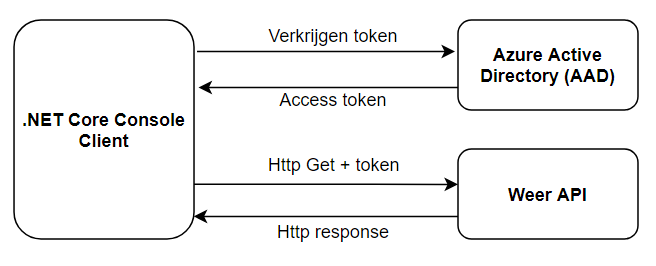
\includegraphics{POC_Final} 
	\caption[Dit is het eindresultaat van dit hoofdstuk]{Dit is het eindresultaat van dit hoofdstuk.}
	\label{fig:pocfinal}
\end{figure}
In deze proof of concept wordt gebruik gemaakt van:	
\begin{itemize}
	\item NET Core SDK 3.1
	\item Text Editor (recommended VS code)
	\item Azure Account (Free)
\end{itemize}
\subsection{\IfLanguageName{dutch}{Aanmaken API}{Making the API}}
Zoals eerder vermeld wordt er in deze proof of concept gebruik gemaakt van een weervoorspelling api. Om deze te gaan aanmaken kan er gebruik gemaakt worden van een NET Core SDK 3.1 template. Met VS code kan er in de terminal het volgende commando ingegeven worden: \emph{dotnet new webapi -n weerApi}.\newline
Na dit command ziet het schema er als volgt uit (figuur \ref{fig:poc1}). Deze template heeft een simpele controller met een get methode die vijf random weersvoorspellingen zal teruggeven. Het aanmaken van de api houdt dan ook niet meer in dan deze simpele stap.
\begin{figure}[H]
	\centering
	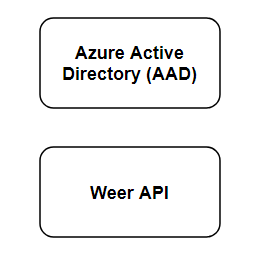
\includegraphics{POC1} 
	\caption[BeginPOC]{Begin vorm van de proof of concept.}
	\label{fig:poc1}
\end{figure}
\subsection{\IfLanguageName{dutch}{Api registreren op Azure}{Registering the API on Azure}}
Nu de api aangemaakt is moet deze bekend gemaakt worden aan Azure active directory. Om dit te doen wordt gebruikt gemaakt van het Azure portal. In het overzicht gaat de gebruiker naar Azure active directory (figuur \ref{fig:azure1}).
\begin{figure}[H]
	\centering
	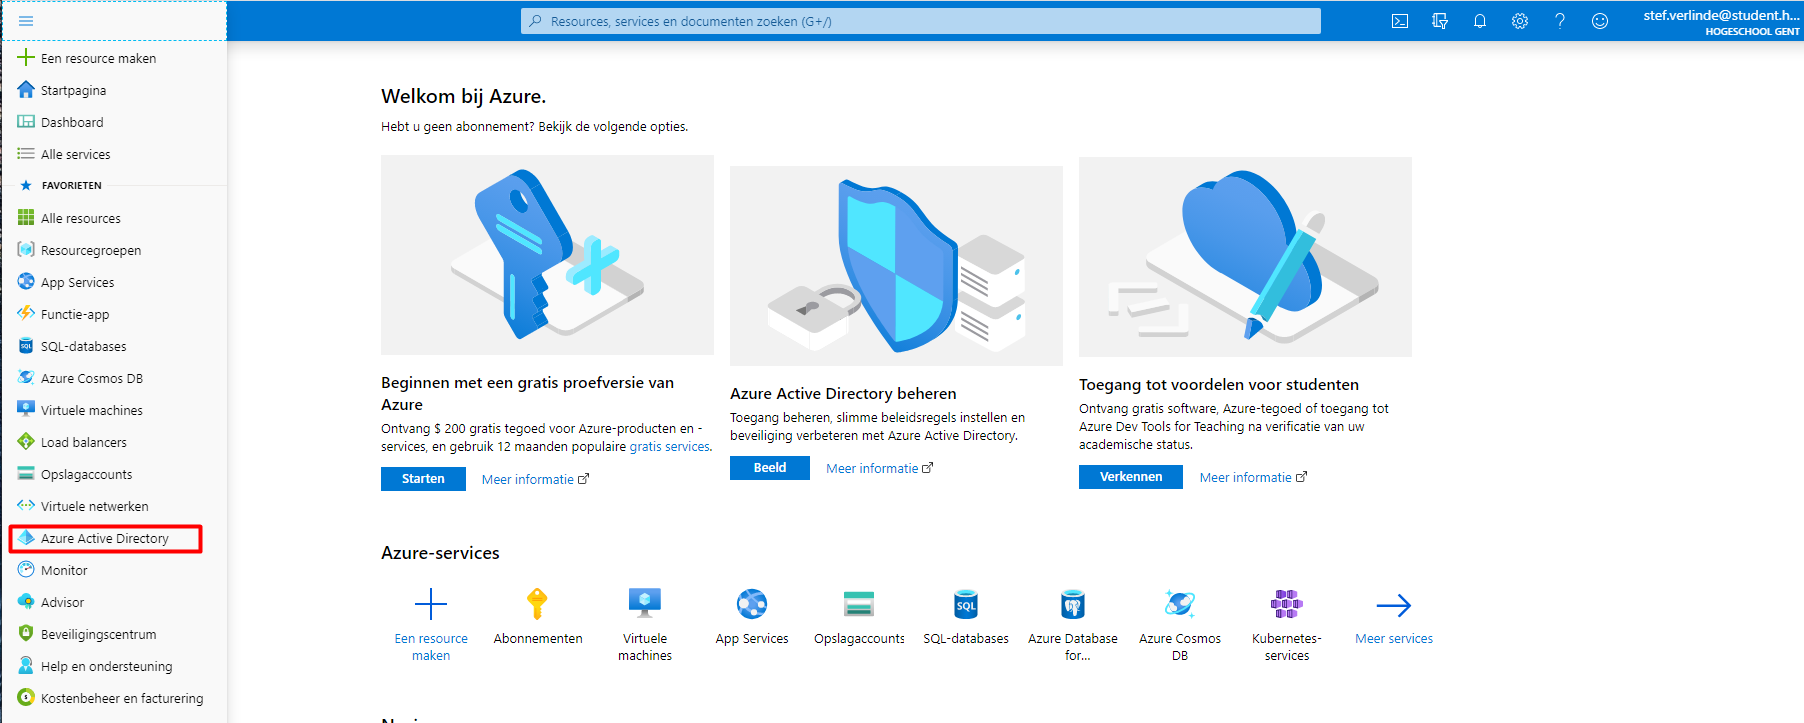
\includegraphics[scale=0.40]{Azure1} 
	\caption[BeginAzure]{Stap 1 in het toevoegen van de API.}
	\label{fig:azure1}
\end{figure}
Om de weer api te registreren bij de active directory wordt in het overzicht genavigeerd naar “App-registraties” (figuur \ref{fig:azure2}).
\begin{figure}[H]
	\centering
	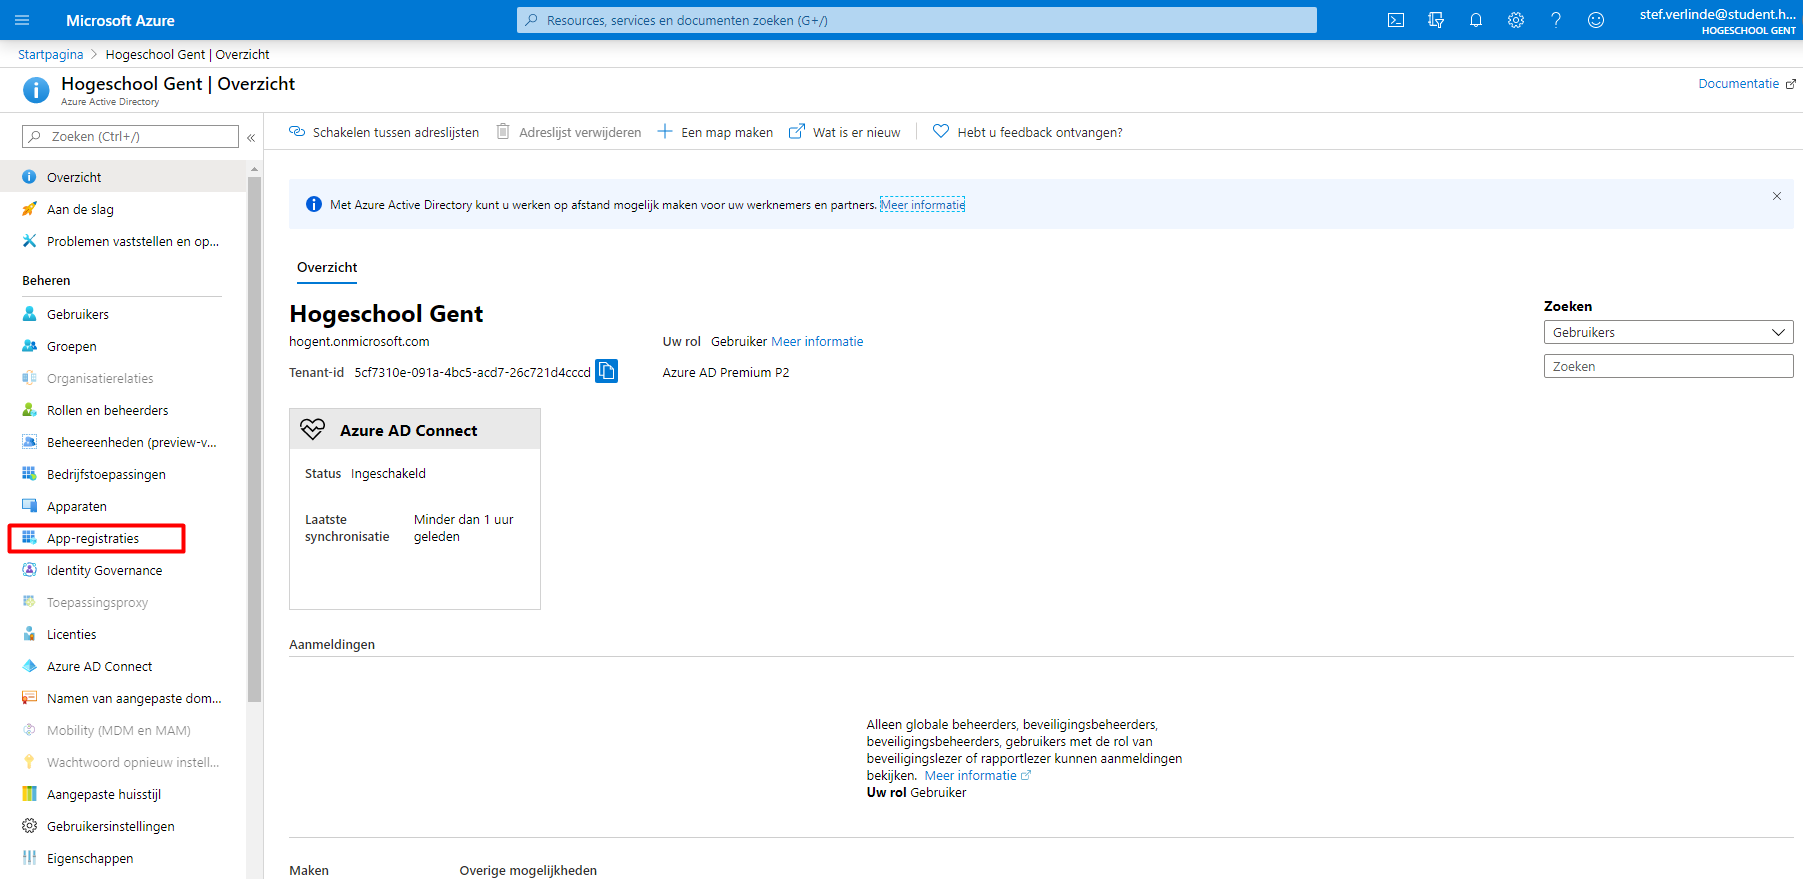
\includegraphics[scale=0.40]{Azure2} 
	\caption[Azure2]{Stap 2 in het toevoegen van de API.}
	\label{fig:azure2}
\end{figure}
In dit overzicht hebben gebruikers de mogelijkheid nieuwe apps te gaan registeren. Hier wordt dus via de knop “Nieuwe registratie” de weervoorspelling api toegevoegd (figuur \ref{fig:azure3}).
\begin{figure}[H]
	\centering
	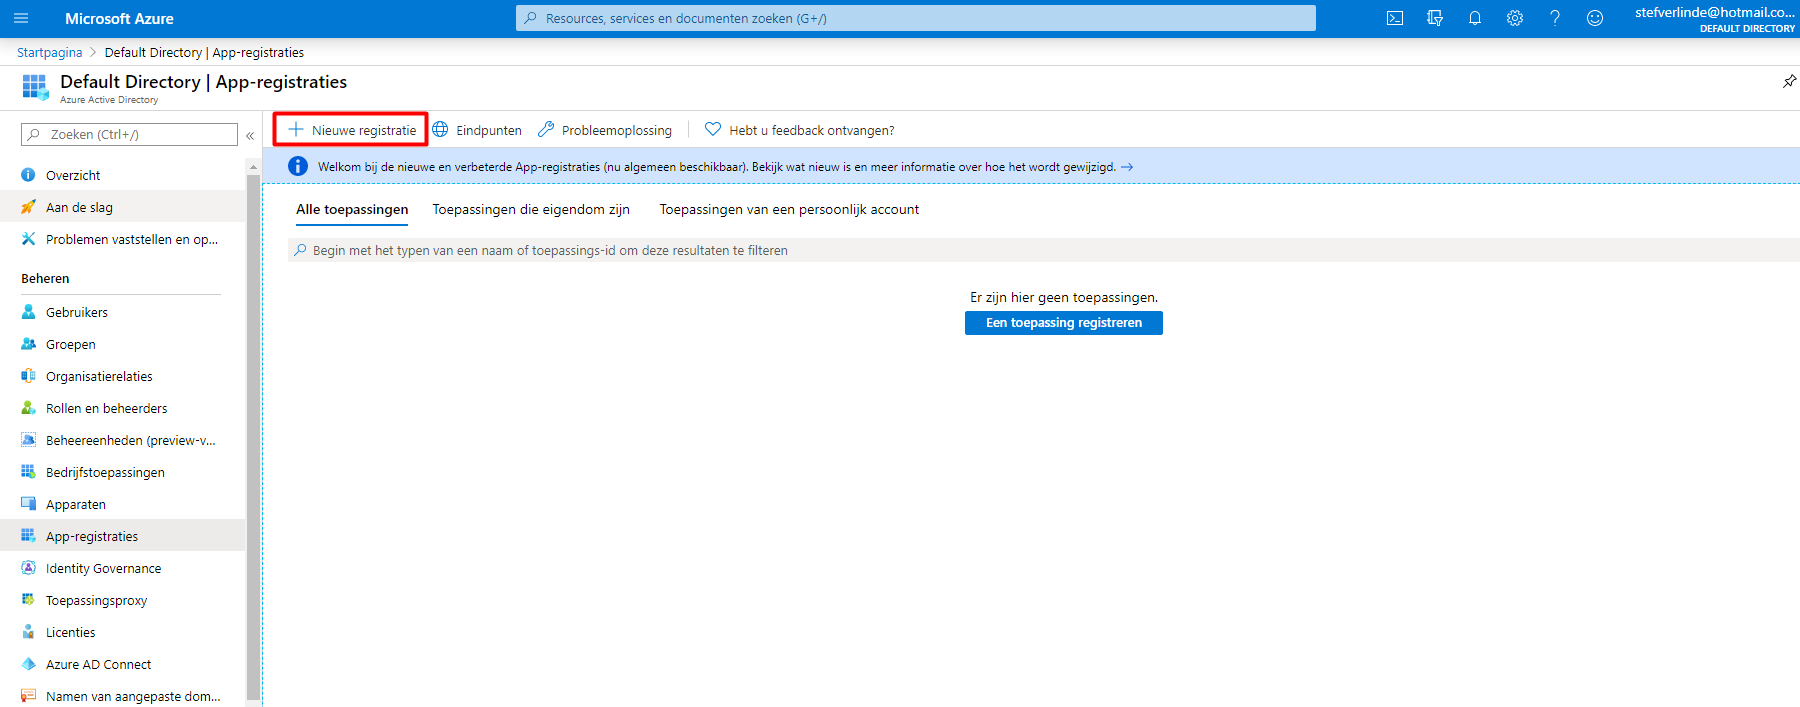
\includegraphics[scale=0.40]{Azure3} 
	\caption[Azure3]{Stap 3 in het toevoegen van de API.}
	\label{fig:azure3}
\end{figure}
In het volgende scherm krijgt de gebruiker de mogelijkheid om een naam in te geven voor de applicatie. In dit geval vult de gebruiker hier in “weerApi”. De overige instellingen eventueel aangepast worden als de gebruiker wenst dat de api ook toegankelijk is voor accounts buiten de directory, bijvoorbeeld bij business-to-business situatie. Hier kan ook een redirect-uri of omleidings-uri opgegeven worden. Als hier een uri wordt opgegeven dan wordt na dat een user geverifieerd is het verificatie antwoord naar deze uri gestuurd, dit wordt bijvoorbeeld gebruikt in de tweede proof of concept. In de applicatie naar applicatie situatie kunnen alle extra instellingen op de standaard waarden gelaten worden. Dit is te zien in figuur \ref{fig:azure4}
\begin{figure}[H]
	\centering
	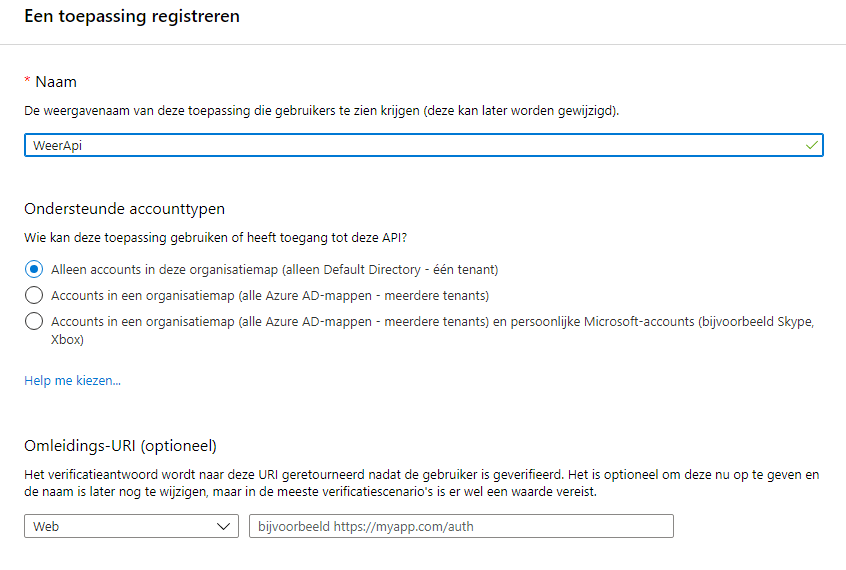
\includegraphics[scale=0.75]{Azure4} 
	\caption[Azure4]{Stap 4 in het toevoegen van de API.}
	\label{fig:azure4}
\end{figure}\newpage
Wanneer de api geregistreerd is binnen de active directory zijn er enkele belangrijke waarden die zichtbaar worden. Deze zijn de client ID en tenant ID. De client ID is een unieke guid voor de api die net geregistreerd werd. De tenant ID is een unieke guid voor onze active directory. Als een gebruiker binnen dezelfde active directory meerdere applicaties zou registreren dan zal deze tenant ID bij elke applicatie dezelfde zijn. Deze waarden zie je in figuur \ref{fig:azure5}.
\begin{figure}[H]
	\centering
	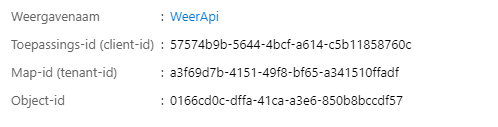
\includegraphics{Azure5} 
	\caption[Azure5]{Belangrijke waarden na het aanmaken van de API.}
	\label{fig:azure5}
\end{figure} 
De volgende stap is het aanmaken van een application ID of resource ID. Dit wordt gedaan om aan Azure duidelijk te maken dat deze api gebruikt zal worden. De api wordt geëxposeerd of beschikbaar gemaakt aan Azure (figuur \ref{fig:azure6}).
\begin{figure}[H]
	\centering
	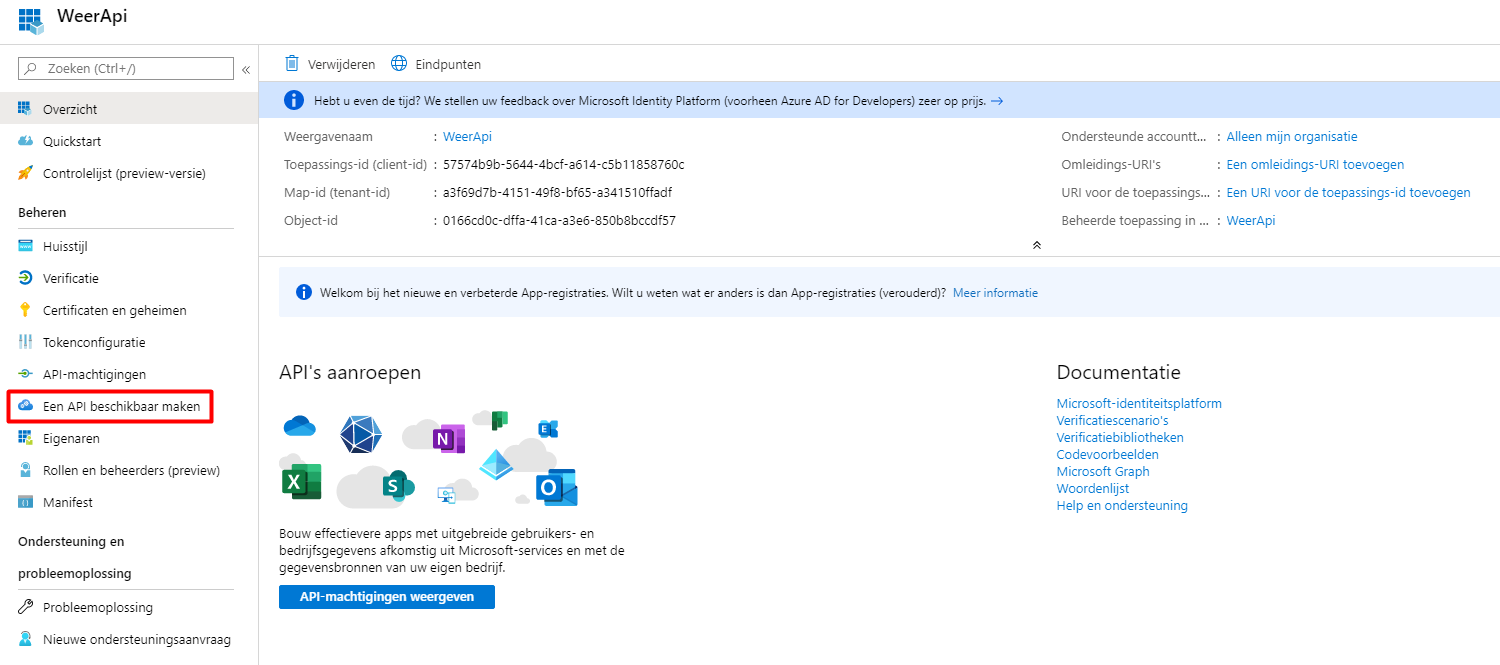
\includegraphics[scale=0.50]{Azure6} 
	\caption[Azure6]{Stap 5 in het toevoegen van de API.}
	\label{fig:azure6}
\end{figure}
Bij “Een api beschikbaar stellen” wordt op de knop “instellen” geklikt en daarna op “opslaan”. Deze stappen worden afgebeeld in figuur \ref{fig:azure7} en \ref{fig:azure8}. Hierdoor wordt er een resource ID aangemaakt. Dit resource ID is nu ook zichtbaar in het overzicht van de api applicatie (figuur \ref{fig:azure9}).
\begin{figure}[H]
	\centering
	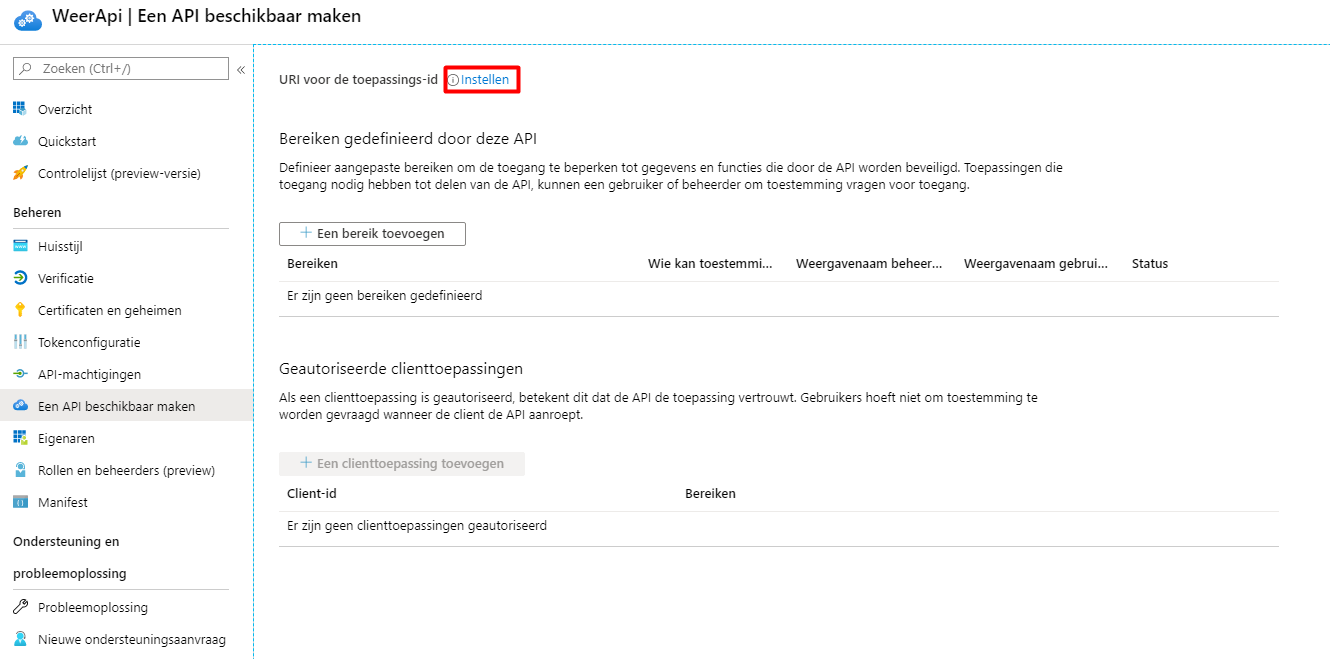
\includegraphics[scale=0.50]{Azure7} 
	\caption[Azure7]{Stap 6 in het toevoegen van de API.}
	\label{fig:azure7}
\end{figure}
\begin{figure}[H]
	\centering
	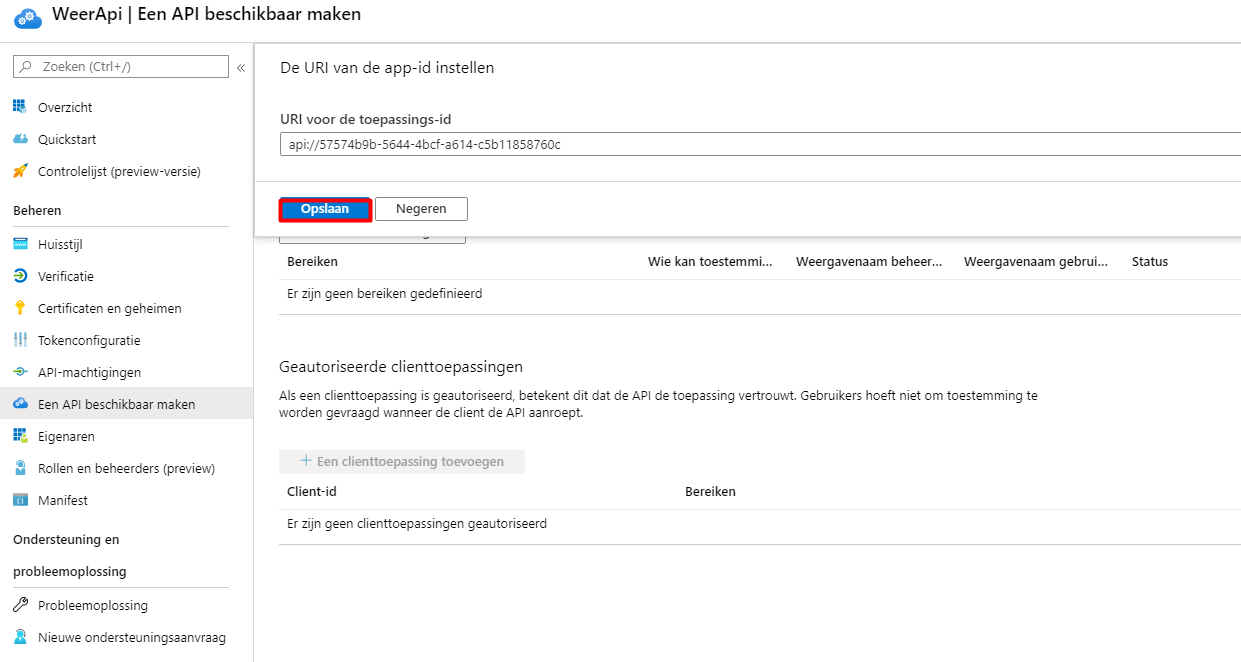
\includegraphics[scale=0.50]{Azure8} 
	\caption[Azure8]{Stap 7 in het toevoegen van de API.}
	\label{fig:azure8}
\end{figure}
\begin{figure}[H]
	\centering
	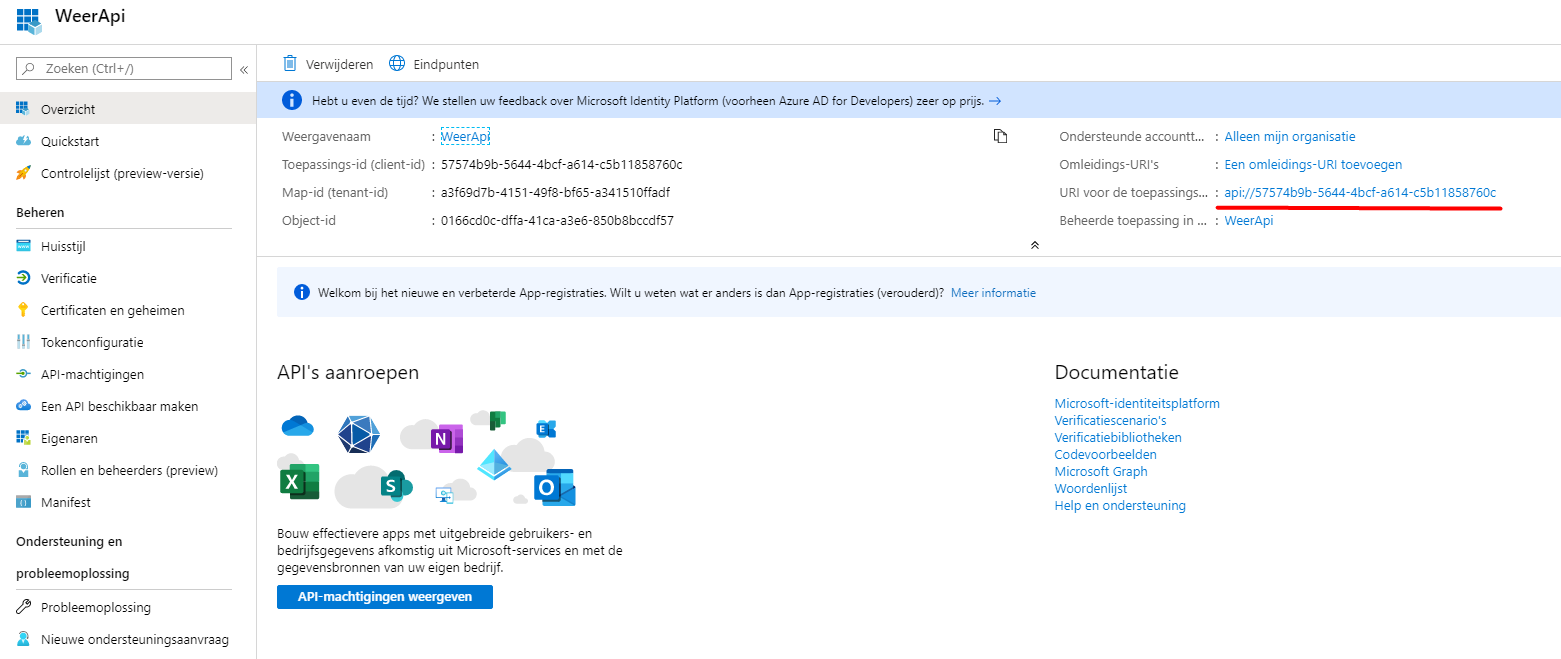
\includegraphics[scale=0.40]{Azure9} 
	\caption[Azure9]{Hier wordt nu het resource ID getoond.}
	\label{fig:azure9}
\end{figure}\newpage
De laatste stap in het registreren van de api applicatie is het wijzigen van het manifest. Een manifest is niks meer dan een json file. In deze json file kan een gebruiker aan Azure vertellen wat voor type applicatie toegang heeft tot de api. \newline
In deze json file zal de gebruiker de “appRoles” array moeten aanpassen zoals in figuur \ref{fig:azure10}. Hier kan een gebruiker verschillende configuratie ingeven. Belangrijk hier is dat ID een geldige guid moet zijn. De waarde voor value is welke applicatie role toegang krijgt tot de api.
\begin{figure}[H]
	\centering
	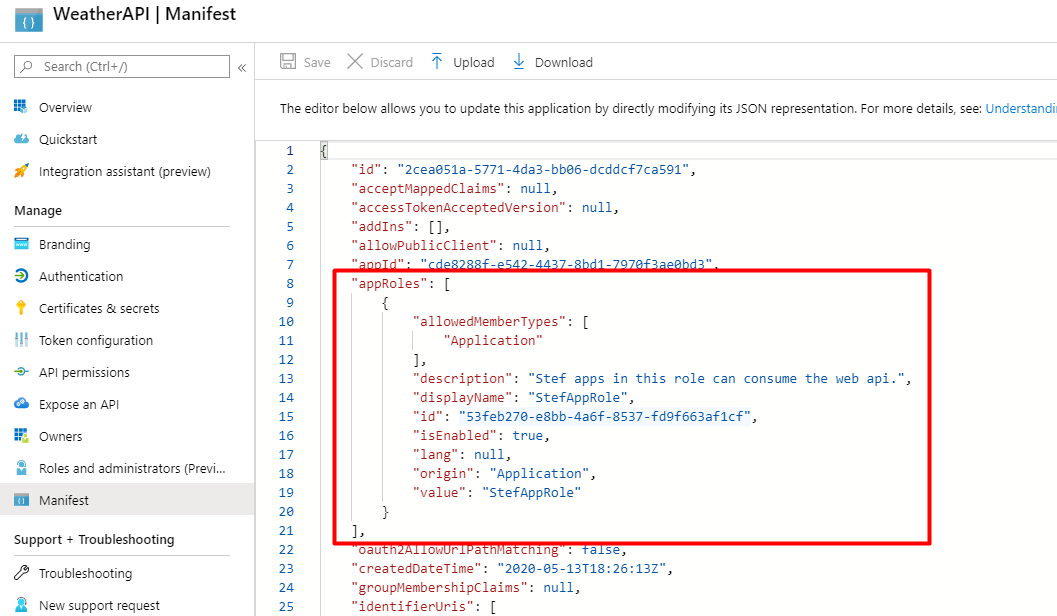
\includegraphics[scale=0.60]{Azure10} 
	\caption[Azure10]{Stap 8 in het toevoegen van de API.}
	\label{fig:azure10}
\end{figure}
\subsection{\IfLanguageName{dutch}{Connectie API en AAD}{Connection API and AAD}}
Nu de api geregistreerd is in Azure active directory kan de gebruiker de momenteel nog aparte api implementatie en registratie op Azure verbinden. Dit gebeurt door het resource ID, tenant ID en instance ID van de Azure api op te slaan in de api implementatie. Voor demonstratie doeleinde worden deze hier opgeslagen in de appsettings.json van het api project (figuur \ref{fig:appsetAPI}). Als de gebruiker wenst deze proof of concept in development te gaan gebruiken wordt aangeraden deze gevoelige informatie in een user secret of key vault te plaatsen.
\begin{figure}[H]
	\centering
	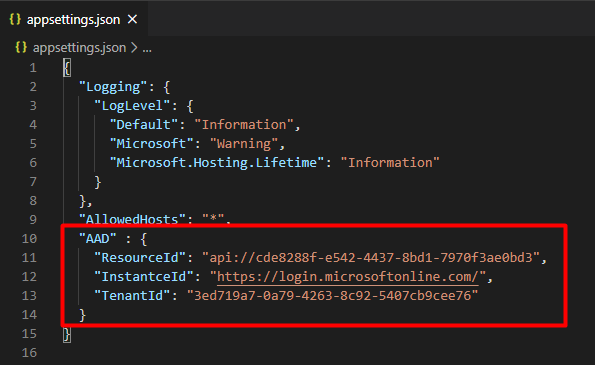
\includegraphics{appsettingsApi} 
	\caption[Appsetingsjosn]{Appsettings.json file van de API.}
	\label{fig:appsetAPI}
\end{figure}
Deze waarden kunnen nu gebruikt worden om de connectie tussen de implementatie en Azure registratie te voltooien. Aangezien de beveiliging van de api aan de hand van jwt bearer tokens gebeurt gebruikt men het resource ID als audience en de instance en tenant ID’s als authority. De code voor in de startup classe zie je in figuur \ref{fig:configureServices} en \ref{fig:configure}. 
\begin{figure}[H]
	\centering
	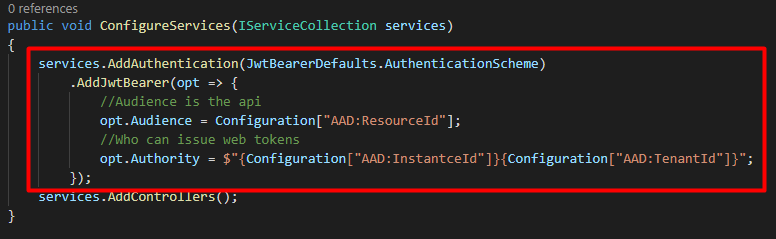
\includegraphics{ConfigureServices} 
	\caption[ConfigureServices]{ConfigureServices methode van de API.}
	\label{fig:configureServices}
\end{figure}\newpage
\begin{figure}[H]
	\centering
	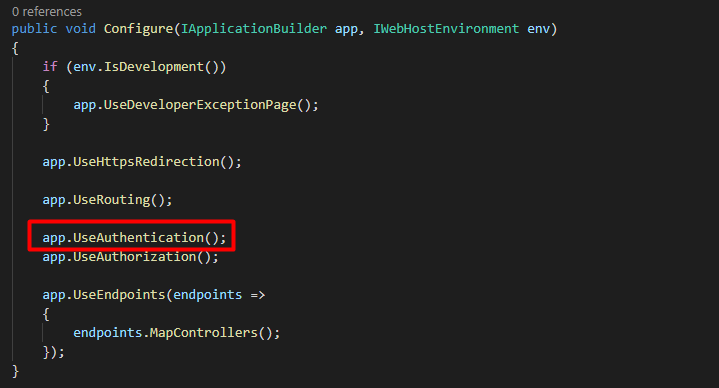
\includegraphics{Configure} 
	\caption[Configure]{Configure methode van de API.}
	\label{fig:configure}
\end{figure}
Laatste stap is het toevoegen van een Authorize attribute aan de endpoint methode. Zo kan deze methode enkel aangeroepen worden door een geverifieerde client. Een niet geverifieerde client krijgt dan een 401 unauthorized error.
\subsection{\IfLanguageName{dutch}{Client registreren op azure}{Registering client on Azure}}
Op een gelijkaardige manier kan ook een client geregistreerd worden bij Azure. In het overzicht “App-registraties” van Azure active directory kan men nu een nieuwe client toevoegen (figuur \ref{fig:azure11}).
\begin{figure}[H]
	\centering
	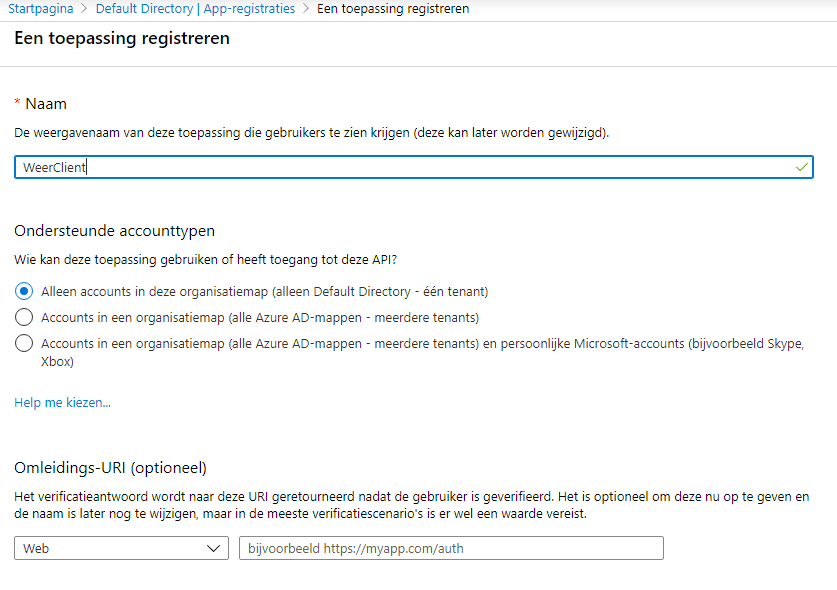
\includegraphics[scale=0.60]{Azure11} 
	\caption[Azure11]{Stap 1 in het registreren van de client.}
	\label{fig:azure11}
\end{figure}
Na het aanmaken van deze client worden de client en tenant ID’s weer zichtbaar, hier valt op dat zoals eerder vermeld het tenant ID dezelfde is als bij de weerApi. De volgende stap is het opzetten van een client secret. Een client secret wordt door de client naar Azure gestuurd om te bewijzen dat de client is wie hij zegt dat hij is. Een client secret is discrete informatie en moet voorzichtig mee omgegaan worden. In het active directory overzicht bij “Certificaten en geheimen” kan een secret worden toegevoegd (figuur \ref{fig:azure12} en \ref{fig:azure13}). 
\begin{figure}[H]
	\centering
	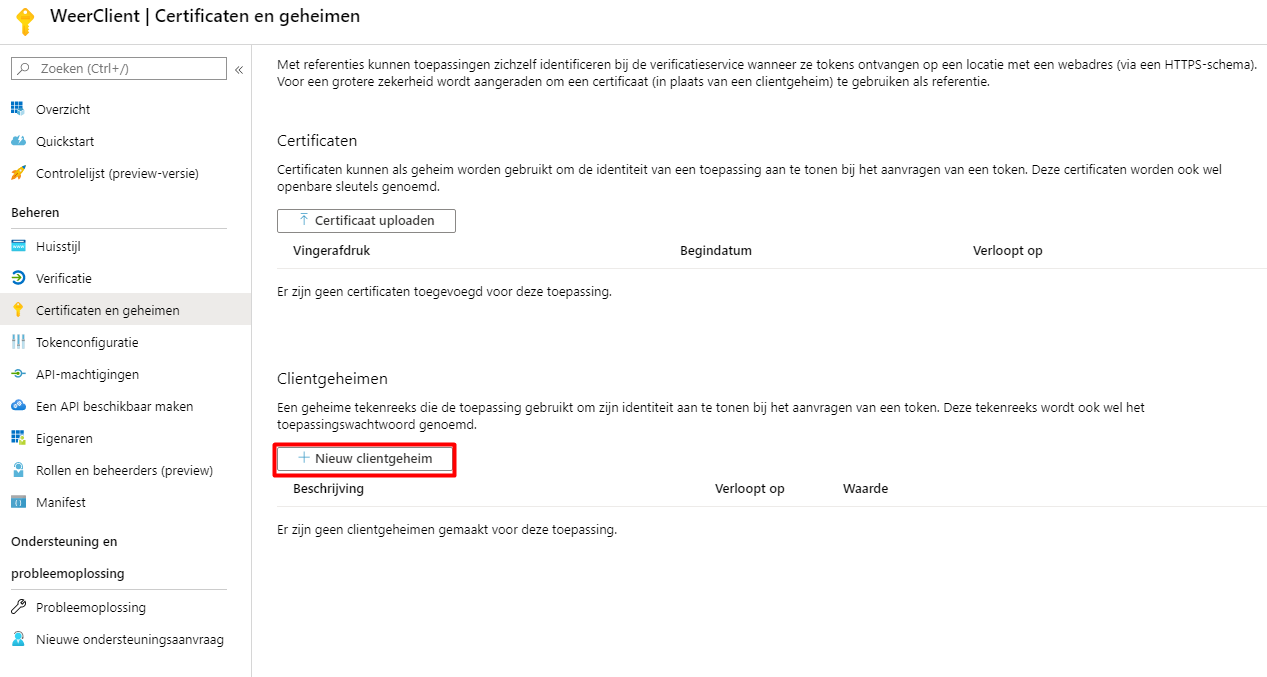
\includegraphics[scale=0.60]{Azure12} 
	\caption[Azure12]{Stap 2 in het registreren van de client.}
	\label{fig:azure12}
\end{figure}
\begin{figure}[H]
	\centering
	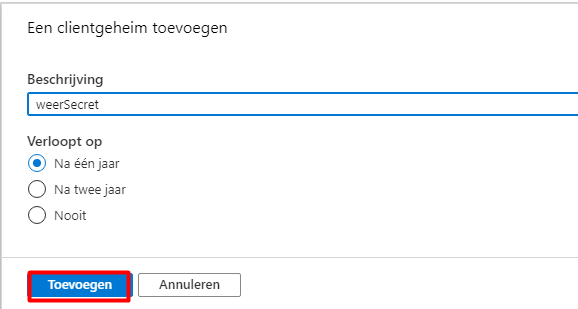
\includegraphics{Azure13} 
	\caption[Azure13]{Stap 3 in het registreren van de client.}
	\label{fig:azure13}
\end{figure}
De laatste stap voor de client is duidelijk maken welke machtigingen de client heeft tegenover de api. Dit kan ingesteld worden via het overzicht “API-machtigingen”. Bij het klikken op machtiging toevoegen valt op dat onder “mijn API’s” de zelf aangemaakte api van de gebruiker terug te vinden is. Na het klikken op de api valt op dat er een keuze is tussen twee machtigingen, gedelegeerde machtigingen en toepassingsmachtigingen. Aangezien er in deze proof of concept een daemon client gebruikt wordt, ofwel een client zonder input van een gebruiker, kiezen we voor toepassingsmachtigingen. Hierna wordt op de role geklikt die in de manifest json file van de api geconfigureerd is (figuur \ref{fig:azure14}). 
\begin{figure}[H]
	\centering
	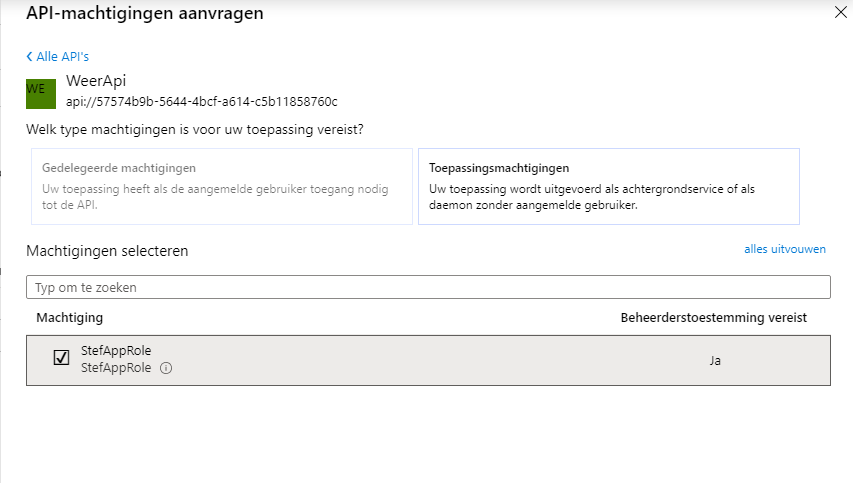
\includegraphics[scale=0.85]{Azure14} 
	\caption[Azure14]{Stap 4 in het registreren van de client.}
	\label{fig:azure14}
\end{figure}
Na het toevoegen van de machtiging is er nog toestemming van de beheerder nodig om deze machtiging te activeren. Dit wordt gedaan door op “Beheerderstoestemming verlenen voor Default Directory” te klikken (figuur \ref{fig:azure15}).
\begin{figure}[H]
	\centering
	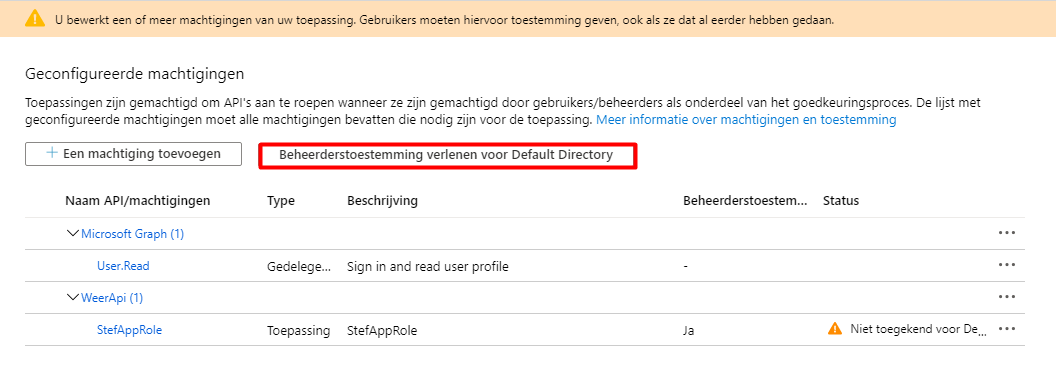
\includegraphics[scale=0.75]{Azure15} 
	\caption[Azure15]{Stap 5 in het registreren van de client.}
	\label{fig:azure15}
\end{figure}
\subsection{\IfLanguageName{dutch}{Aanmaken client application}{Making the client application}}
Gelijkaardig aan de api is het mogelijk met het volgende dotnet commando een console applicaite template genereren: \emph{dotnet new console -n weerClient}\newline
Schematisch wordt de flow na het aanmaken van de client als volgt afgebeeld (figuur \ref{fig:poc2}). Alles in Azure active directory staat al klaar voor de communicatie maar hiervoor moet de configuratie in de client in orde gebracht worden.
\begin{figure}[H]
	\centering
	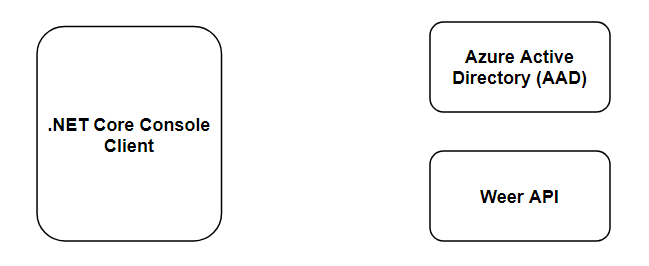
\includegraphics{POC2} 
	\caption[POC2]{Na het maken van de client kan het schema als volgt worden aangevuld.}
	\label{fig:poc2}
\end{figure}
Net zoals in de api applicatie is het belangrijk dat de client op de hoogte is van enkele waarden uit Azure active directory. Deze zijn de instance, tenant ID, client ID, de gemaakte client secret en het basis adres van de api (figuur \ref{fig:appsettingsClient}). In dit voorbeeld ziet dit er als volg uit. Ook hier is het belangrijk om te begrijpen dat dit enkel in appsettings wordt opgeslagen voor demonstratiedoeleinden. In een development omgeving zouden client secrets in een key vault opgeslagen worden.
\begin{figure}[H]
	\centering
	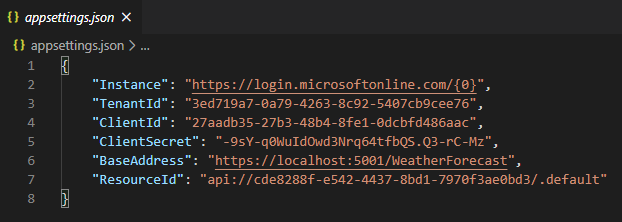
\includegraphics{appsettingsClient} 
	\caption[POC2]{appsettings.json file in de client applicatie.}
	\label{fig:appsettingsClient}
\end{figure}
Omdat appsettings een json bestand is heeft de console applicatie een manier nodig om deze te kunnen inlezen. Om dit te vergemakkelijken maken wordt er een AuthConfig klasse aan gemaakt met alle attributen die nodig zijn voor de Azure connectie te maken (figuur \ref{fig:authConfig}).
\begin{figure}[H]
	\centering
	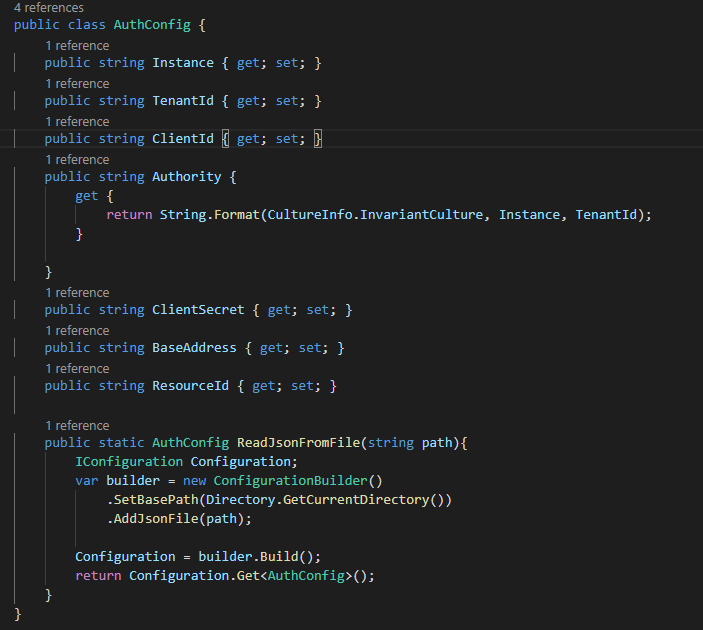
\includegraphics{AuthConfig} 
	\caption[AuthConfig]{AuthConfig klasse in de client.}
	\label{fig:authConfig}
\end{figure}\newpage
Vanaf nu is alles aanwezig om een connectie met Azure te maken. In dit voorbeeld doen we dit als volgt. De eerste connectie die de client moet is een geldige token vragen aan Azure active directory. In figuur \ref{fig:aquireToken} zien we dat eerst de waarden uit het appsetings bestand gelezen worden, daarna wordt een ConfidentialClient aangemaakt met het voorziene client ID, client secret en de authority. Er is ook een array van resource ID’s. Deze heeft in dit voorbeeld enkel de weer Api als resource vandaar dat hier het resource ID van deze api inkomt. De volgende try block haalt de token op voor de client van de resource en print deze uit.
\begin{figure}[H]
	\centering
	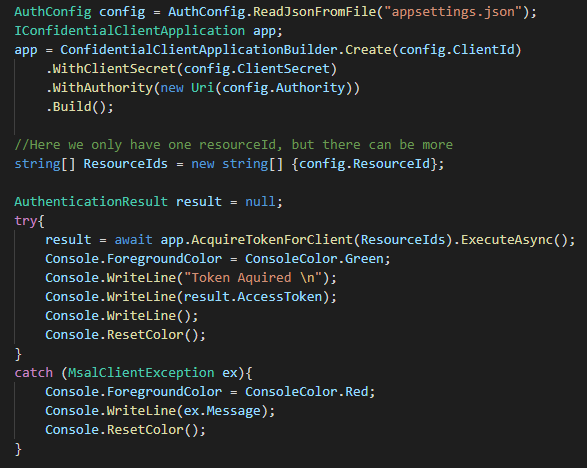
\includegraphics{AquireToken} 
	\caption[AuthConfig]{Deze code toont het ophalen van de access token door de client.}
	\label{fig:aquireToken}
\end{figure}\newpage
Na het uitvoeren van deze code is volgende connectie succesvol gelegd. Een client in dit geval de weer client kan nu een access token ophalen van de Azure active directory.
\begin{figure}[H]
	\centering
	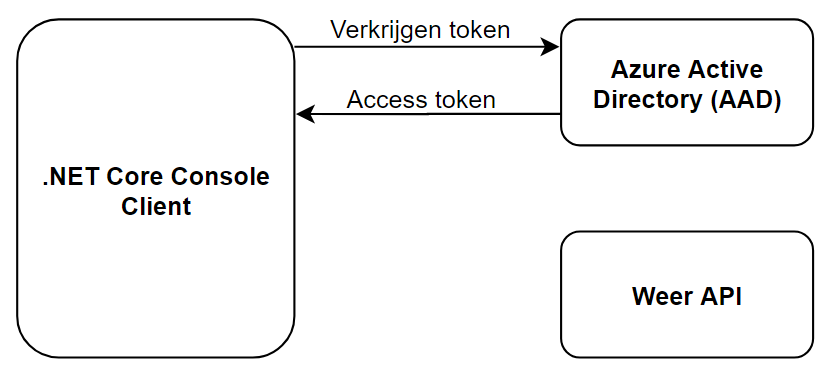
\includegraphics[scale=0.60]{POC3} 
	\caption[POC3]{Hier wordt schematisch afgebeeld dat de client nu een access token van AAD kan ophalen.}
	\label{fig:poc3}
\end{figure}
Om het schema compleet te maken moet de client met deze access token om de api data vragen. Als deze access token correct is zal de client de weer gegevens krijgen. In deze proof of concept gebeurt dit als volgt.\newline
Als eerste wordt gecheckt of er een access token van Azure active directory aanwezig is. Daarna wordt er een httpClient aangemaakt en wordt er gecheckt of de defaultRequestHeaders het media type json accepteren. Daarna wordt het autorisatie type op bearer gezet en wordt er een get methode naar de api gestuurd. Als de response succesvol is word deze uitgeprint, anders de error (figuur \ref{fig:aquireData}).
\begin{figure}[H]
	\centering
	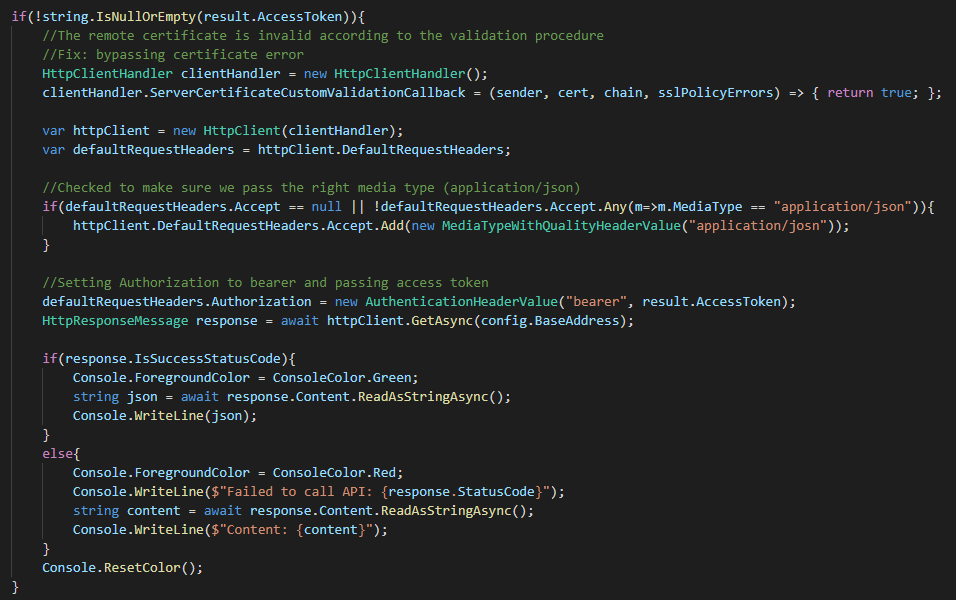
\includegraphics[scale=0.73]{AquireData} 
	\caption[AquireData]{Deze code toont het ophalen van data aan de hand van een access token op de API.}
	\label{fig:aquireData}
\end{figure}\newpage
Door deze code is het schema compleet en kan de client met een access token van Azure active directory aan de data van de api.
\begin{figure}[H]
	\centering
	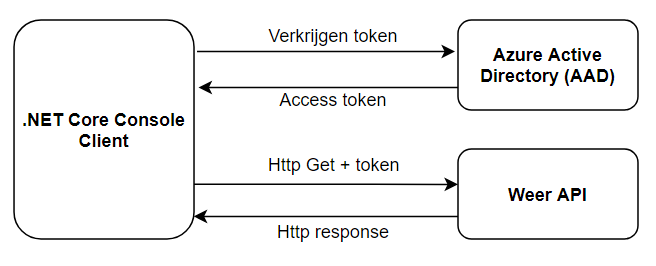
\includegraphics{POC_Final} 
	\caption[POCFinal2]{Op dit schema is het eindresultaat te zien.}
	\label{fig:pocfinal2}
\end{figure}
\section{\IfLanguageName{dutch}{Password grant}{Password grant}}
\label{sec:Microsift_signon}
Het verschil met sign-on authenticatie en application to application authenticatie is dat er bij sign-on input van de gebruiker verwacht wordt. Namelijk een gebruikersnaam en wachtwoord, hierdoor zijn er enkele extra stappen in de flow voor de authenticatie. Bij application to application is er geen input van de gebruiker, zoals gezien in de eerste proof of concept.
\subsection{\IfLanguageName{dutch}{Registratie in azure}{Registration in Azure}}
Om een client met sign-on authenticatie toe te voegen aan de Azure active directory gaat de gebruiker naar “App-registraties” in de Azure portal bij active directory. Hier wordt weer een nieuwe client toegevoegd met de knop “Nieuwe registratie”. Als naam wordt hier “SignOnClient” genomen, de andere instellingen houden we op de default instellingen (figuur \ref{fig:azure16}). 
\begin{figure}[H]
	\centering
	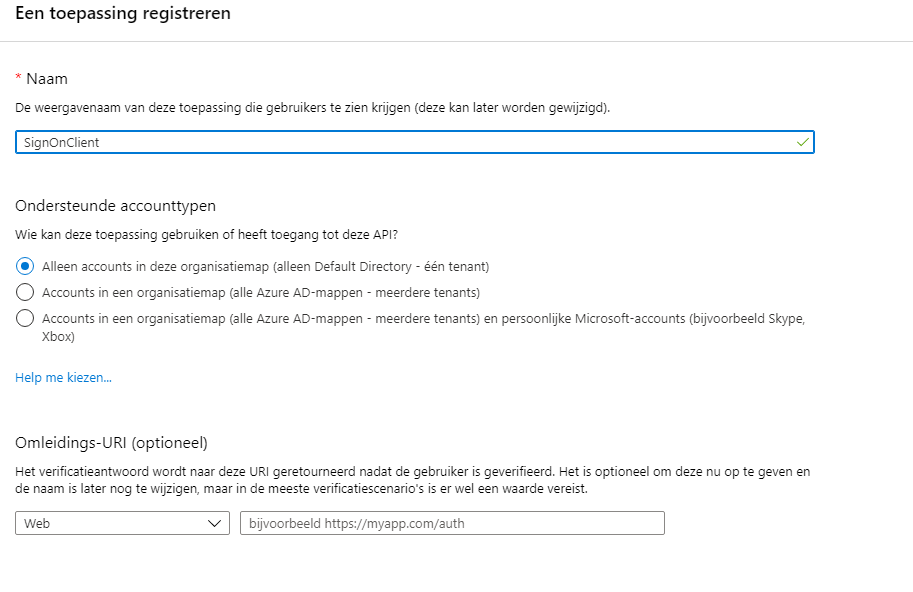
\includegraphics[scale=0.75]{Azure16} 
	\caption[Azure16]{Stap 1 in het registreren van de client met password grant.}
	\label{fig:azure16}
\end{figure}
Na het aanmaken van de client is het mogelijk om bij ”Quickstart” makkelijk de client te configureren. Hier worden er enkele mogelijkheden voorgesteld door Azure voor het opstarten van de client. In deze proof of concept werd er gekozen voor een .NET Core webtoepassing (figuur \ref{fig:azure17} en \ref{fig:azure18}).
\begin{figure}[H]
	\centering
	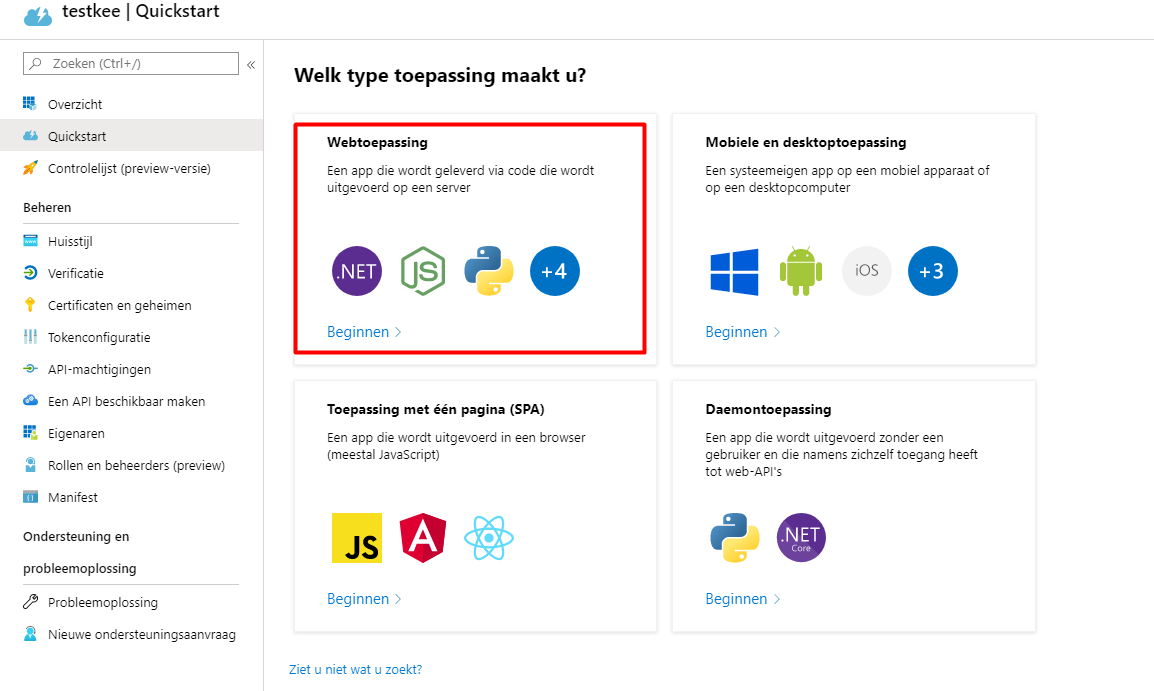
\includegraphics[scale=0.60]{Azure17} 
	\caption[Azure17]{Stap 2 in het registreren van de client met password grant.}
	\label{fig:azure17}
\end{figure}\newpage
\begin{figure}[H]
	\centering
	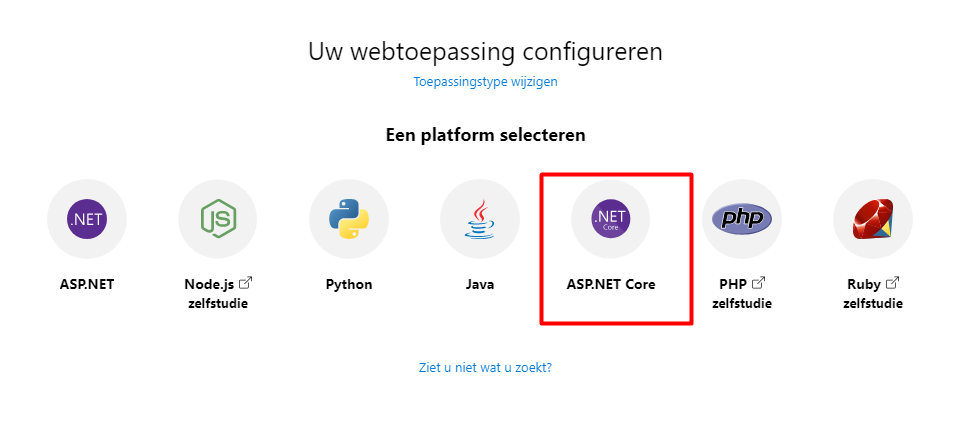
\includegraphics[scale=0.60]{Azure18} 
	\caption[Azure18]{Stap 3 in het registreren van de client met password grant.}
	\label{fig:azure18}
\end{figure}
In het laatste scherm van de quickstart worden er door Azure enkele stappen voorgelegd. Bij stap 1 moeten er enkele URLs opgegeven worden, dit zijn de redirect URLs en postLogout URLs. Onder deze stap is er ook een knop om dit Azure automatisch te laten doen zodat de gebruiker dit zelf niet moet invullen. Deze automatische invulling is ook wat in deze proof of concept gebruikt is. Stap 2 is om de quickstart te downloaden. Na het downloaden en starten van de client zou het inloggen met een Microsoft-account al moeten werken.\newline
Het verschil tussen een sign-on authenticatie en application to appliction authenticatie bevindt zicht dus in de flow van de tokens. Zoals in het schema van de flow gezien wordt zijn er bij sign-on enkele extra stappen verijst. In deze proof of concept wordt er eerst naar de .NET Core applicatie gegaan, maar het request zal meteen doorgestuurd worden naar de Microsoft identity server. Hier zal de gebruiker zijn gegevens moeten ingeven om zo aan een geldige access token te komen. Na deze stap wordt met de redirectURL teruggegaan naar de .NET Core applicatie en kan de pagina geladen worden. Omdat we bij het aanmaken van de client in Azure ervoor gekozen hebben dat deze client enkel toegankelijk mocht zijn voor users binnen de organisatiemap zullen enkel Microsoft accounts binnen de Azure active directory toegang hebben na het inloggen. Een schematische voorstelling van de token flow kan gezien worden in figuur \ref{fig:signOn}. 
\begin{figure}[H]
	\centering
	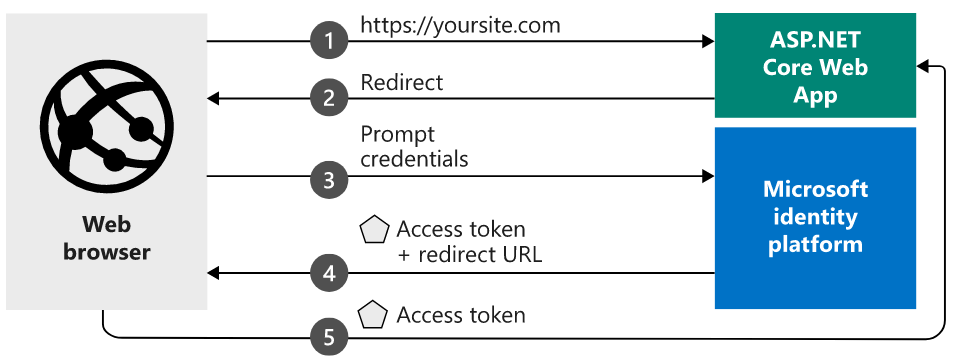
\includegraphics[scale=0.80]{SignOn} 
	\caption[SignOn]{Schematische voorstelling van de password grant flow.}
	\label{fig:signOn}
\end{figure}